Today, we introduce the non-linear dimensionality reduction method
t-distributed Stochastic Neighbor Embedding (tSNE), a method widely
used in high-dimensional data visualization and exploratory
analysis. We will go over how the method was developed over years, its
limitations, and briefly the recent theoretical guarantees on the
algorithm. 

\section{Introduction to tSNE}
\subsection{Timeline}
\begin{center}
    \begin{tabular}{ | l | l | p{5cm} | p{5cm} |}
    \hline
    \textbf{Year} & \textbf{Method} & \textbf{Author} & \textbf{Summary} \\ \hline
    1901 & PCA & Karl Pearson & First dimensionality reduction technique \\ \hline
    2000 & Isomap & Tenenbaum, de Silva, and Langford & First non-linear dimensionality reduction technique \\ \hline
    2002 & SNE & Hinton and Roweis & Original SNE algorithm \\ \hline
    2008 & tSNE & Maaten and Hinton & Addressed the crowding issue of SNE, $O(N^2)$ \\ \hline
    2014 & BHt-SNE & Maaten & Using Barnes–Hut approximation to achieve $O(N\log(N))$ \\ \hline
    2017 & & Linderman and Steinerberger & First step towards theoretical guarantee for t-SNE \\ \hline
    2017 & Fit-SNE & Linderman et al. & Acceleration to $O(N)$ \\
    \hline
    2018 & & Arora et al. & Theoretical guarantee for t-SNE \\ \hline
    2018 & & Verma et al. & Generalization of t-SNE to manifold \\ \hline
    \end{tabular}
\end{center}
\textbf{Open Question:} online t-SNE

\subsection{Motivation}
Most data-sets exhibit non-linear relationship among features and data
points reside in high-dimensional space. Therefore, we want a
low-dimensional embedding of high-dimensional data that preserves the
relationship among different points in the original space in order to
visualize data and explore the inherent structure of data such as
clusters. However, many linear dimensionality methods such as PCA and
classical manifold embedding algorithms such as Isomap fail. Our
technical aim is to embed high-dimensional data to 2-D or 3-D while
preserving the relationships among data points (ie. similar points
remain similar; distinct points remain distinct). 

\subsection{Stochastic Neighbor Embedding (SNE)}
Previous non-linear dimensionality reduction methods have a fixed
assignment in low-dimensional space for a data point in the
high-dimensional space, but this often fails to correctly capture a
portion of the ambiguous points that could belong several to local
neighborhoods. SNE aims to best capture neighborhood identity by
considering the probability that one point is the neighbor of all
other points. It first models a distribution over the neighbors for
each data point, then minimizes the distance between the original 
distribution and the distribution induced by the mapped data points.
Formally, it defines $n\times n$ similarity matrix $P$
in the high dimensional space whose entries are 
\[ p_{j\vert i} = \frac{exp(-\vert \vert x_i -x_j \vert \vert^2 /
  2\tau_i^2)}{\sum_{k\neq i} exp(-\vert \vert x_i -x_k \vert \vert^2 /
  2\tau_i^2)}\] where $\tau_i^2$ is the variance for the Gaussian distribution
  centered around $x_i$, which normalizes the distribution based on the size of
  the neighborhood. And $n\times n$ similarity matrix $Q$ in the low dimensional
  space whose entries are 
\[
q_{j\vert i} = \frac{exp(-\vert \vert y_i - y_j \vert
  \vert^2)}{\sum_{k\neq i} exp(-\vert \vert y_i -y_k \vert \vert^2)} 
\]
Note that we can interpret $p_{j\vert i}$ as the probability that
$x_j$ is a neighbor of $x_i$'s, and $P$ is simply a probability
distribution. Then define the cost function as the Kullback-Leibler
divergence over $P$ and $Q$ 
\[
C=\sum_i KL(P_i \vert \vert Q_i) = \sum_i \sum_j p_{j\vert i} \log
\frac{p_{j \vert i}}{q_{j \vert i}} 
\]
From the definition of $P$, note that SNE focuses on local structure
because farther points result in smaller $p_{ij}$ and closer points
result in greater $p_{ij}$. The gradient of C is 
\[\frac{dC}{dy_i}=2\sum_{j} (y_i-y_j)(p_{j|i}-q_{j|i}+p_{i|j}-q_{i|j}) \]
To choose the appropriate $\tau_i^2$, SNE performs a binary search for
the value of $\tau_i$ that makes the entropy of the distribution over
neighbors equal to $\log(k)$, where $k$ is the hyper-parameter
perplexity or the effective number of local neighbors. The perplexity
is defined as: 
\[
k=2^{H(P_i)}
\]
where $H(P_i)$ is the Shannon entropy of $P_i$ measured in bits:
\[
H(P_i)=-\sum_j p_{j \vert i} \log_2 p_{j \vert i}
\]
Therefore, for denser data, greater perplexity $k$ should be chosen,
which would result in a smaller $\tau_i^2$ and neighborhood
size. Another consequence is that since the Gaussian kernel is used,
the probability of being a neighbor decreases sharply for any point
$x_j$ that lies outside of the neighborhood of a point $x_i$, and the
neighborhood is determined exactly by $\tau_i^2$. 

\begin{center}
    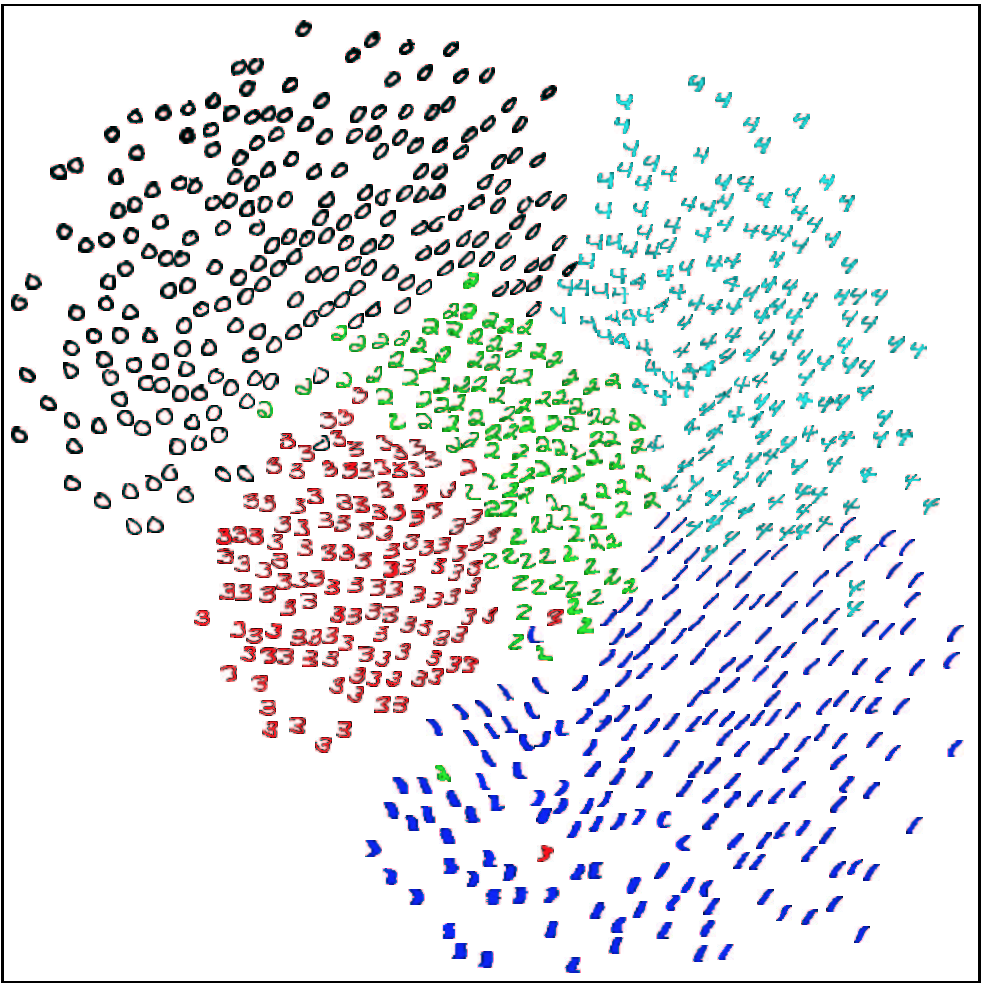
\includegraphics[scale=0.5]{chapter_7/files/fig1.png}
    \captionof{figure}{The result of running the SNE algorithm on 3000 256-dimensional
    gray-scale images of handwritten digits (not all points are shown).}
\end{center}

\noindent As well as SNE preserves local relationships, it suffers
from the "crowding problem". The area of the 2D map that is available
to accommodate moderately distant data points will not be large enough
compared with the area available to accommodate nearby data points.

Intuitively, there is less space in a lower dimension to accommodate moderately distant data points originally in higher dimension. See the following example.

\begin{center}
    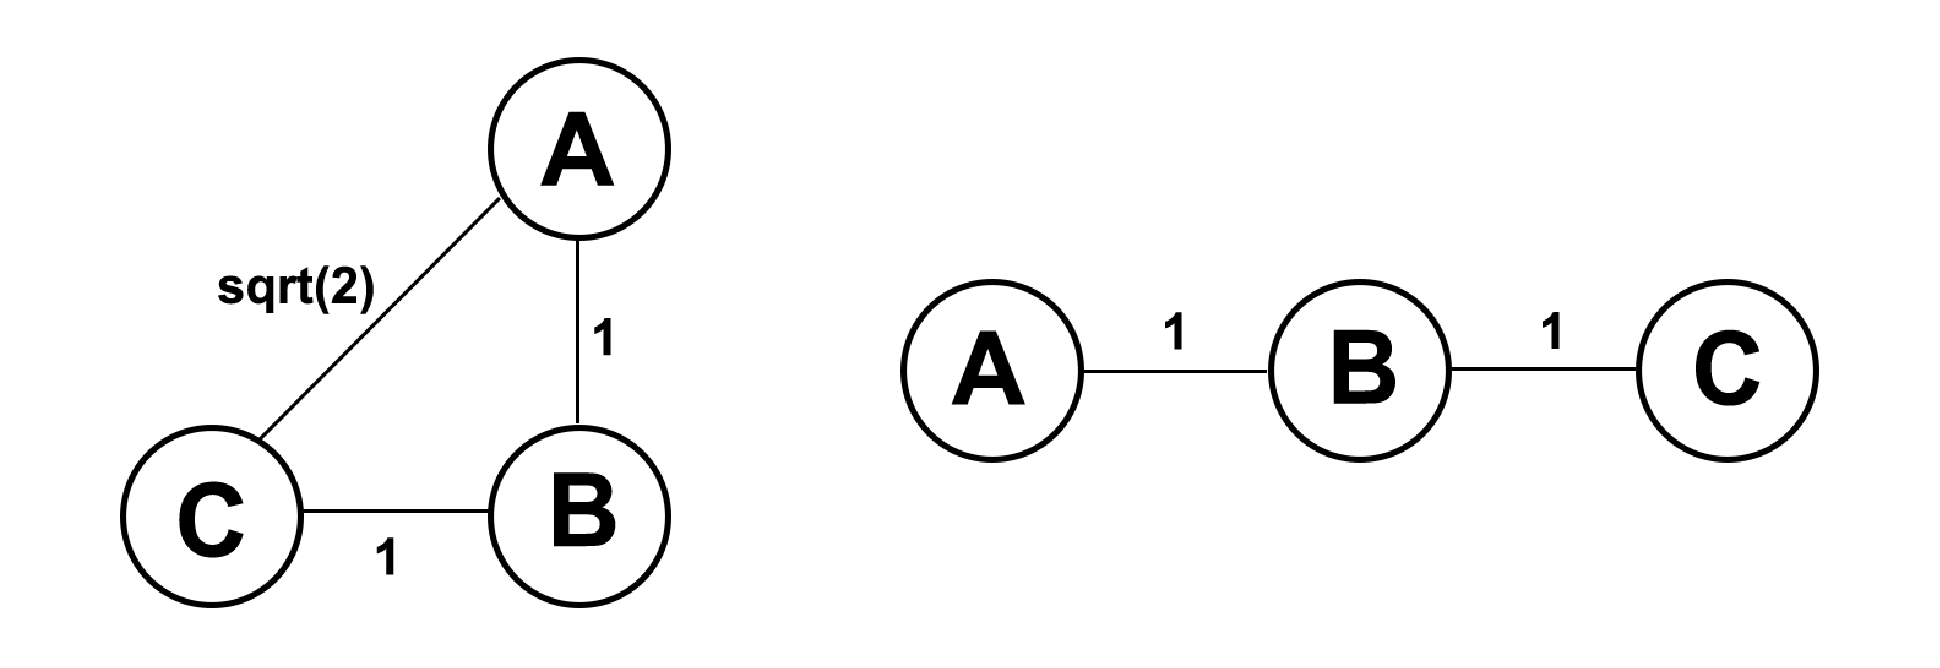
\includegraphics[scale=0.4]{chapter_7/files/fig2.png}
    \captionof{figure}{An embedding from 2D (left) to 1D (right). Although the
      distances between the closest points AB and BC are preserved, the global
      distance AC has to increase. We therefore want to shrink the distances of
      AB and BC by a small amount so that AC is not as distorted}. 
\end{center}

As a result, globally distinct clusters in high dimensional space
would get pushed closer to each other and often times cannot be
distinguished from each other in 2D or 3D embedding. 

\subsection{t-Distributed Stochastic Neighbor Embedding (t-SNE)}
To address the crowding problem and make SNE more robust to outliers, t-SNE was
introduced. Compared to SNE, t-SNE has two main changes: 1) a symmetrized
version of the SNE cost function with simpler gradients 2) a Student-t
distribution rather than a Gaussian to compute the similarity in the
low-dimensional space to alleviate the crowding problem.\\

\noindent Notice that in SNE, $p_{ij}$ is not necessarily equal to
$p_{ji}$, because $\tau_{ij}$ is not necessarily equal to
$\tau_{ji}$. This makes SNE prone to outliers, because an outlier
$x_i$ would have very small $p_{ji}$ for all other points, and so its
embedded location becomes irrelevant. Thus, in t-SNE $p_{ij}$ is
defined instead as 
\[
p_{ij} = \frac{p_{j \vert i}+p_{i \vert j}}{2n}
\]
In this way, $\sum_j p_{ij} > \frac{1}{2n}$ for all data points
$x_i$, and is symmetric for $p_{ij}$ and $p_{ji}$. As a result, each $x_i$ makes a significant contribution to the cost function, and that also gives a simpler gradient, 
as shown later. \\ 

\noindent Moreover, t-SNE uses the Student's t-distribution instead of
the Gaussian to define Q 
\[
q_{ij}=\frac{(1+\vert \vert y_i - y_j \vert \vert^2)^{-1}}{\sum_{k\neq l}(1+\vert \vert y_k - y_l \vert \vert^2)^{-1}}
\]
The cost function of t-SNE is now defined as:
\[
C=\sum_i KL(P_i \vert \vert Q_i) = \sum_{i=1}^n \sum_{j=1}^n p_{ij} \log \frac{p_{ij}}{q_{ij}}
\]
The heavy tails of the normalized Student-t kernel allow dissimilar
input objects $x_i$ and $x_j$ to be modeled by low-dimensional
counterparts $y_i$ and $y_j$ that are far apart because $q_{ij}$ is
would be large for two embedded points that are far apart. 
And since $q$ is what to be learned, the outlier problem does not
exist for low-dimension. \\ 

\noindent The gradient of the cost function is:
\begin{align*}
\frac{dC}{dy_i}
&=4\sum_{j=1, j\neq i}^{n} (p_{ij}-q_{ij})(1+||y_i-y_j||^2)^{-1}(y_i-y_j)\\
&= 4\sum_{j=1, j\neq i}^{n} (p_{ij}-q_{ij})q_{ij}Z(y_i-y_j)\\
&= 4\Big ( \sum_{j \neq i} p_{ij}q_{ij}Z(y_i-y_j)-\sum_{j\neq i}q_{ij}^2 Z(y_i-y_j) \Big )\\
&= 4(F_{attraction}+F_{repulsion})
\end{align*}
where $Z=\sum_{l,s=1, l\neq s}^{n} (1+||y_l-y_s||^2)^{-1}$. The
derivation can be found t-SNE paper's appendix.\\ 

\begin{algorithm}
\caption{tSNE}
\begin{algorithmic} 
\STATE \textbf{Input:} Dataset $X=\{x_1,...,x_n\} \in \mathbb{R}^d$,
perplexity $k$, exaggeration parameter $\alpha$, step size $h>0$,
number of rounds $T \in \mathbb{N}$\; 
\STATE Compute $\{p_ij:i,j\in [n],i\neq j\}$
\STATE Initialize $y_1^{(0)}, y_2^{(0)},...,y_n^{(0)}$ i.i.d. from the
uniform distribution on $[-0.01,0.01]^2$ 
\FOR{t=0 \textbf{to} T-1}
    \STATE $Z^{(t)} \leftarrow \sum_{i,j\in [n],i\neq j}\Big ( 1+ ||y_i^{(t)}-y_j^{(t)}|| \Big )^{-1}$
    \STATE $q_{ij}^{(t)} \leftarrow \frac{\Big ( 1+ ||y_i^{(t)}-y_j^{(t)}|| \Big )^{-1}}{Z^{(t)}}$, $\forall i,j\in [n],i\neq j$
    \STATE $y_i^{t+1}\leftarrow y_i^{(t)}+h\sum_{j\in [n] / \{i\}} \Big (\alpha p_{ij}-q_{ij}^t \Big )q_{ij}^t Z^t\Big (y_i^{(t)}-y_j^{(t)} \Big )$, $\forall i \in [n]$
\ENDFOR
\STATE \textbf{Output:} 2D embedding $Y^{(T)}=\Big\{y_1^{(T)},y_2^{(T)},...,y_n^{(T)} \Big\} \in \mathbb{R}^2$
\end{algorithmic}
\end{algorithm}

Notice that there is an exaggeration parameter $\alpha > 1$ in the
tSNE algorithm, which is used as a coefficient for $p_{ij}$. This
encourages the algorithm to focus on modeling large $p_{ij}$ by fairly
large $q_{ij}$ . A natural result is to form tightly separated
clusters in the map and thus makes it easier for the clusters to move
around relative to each other in order to find an optimal global
organization. 

\begin{center}
    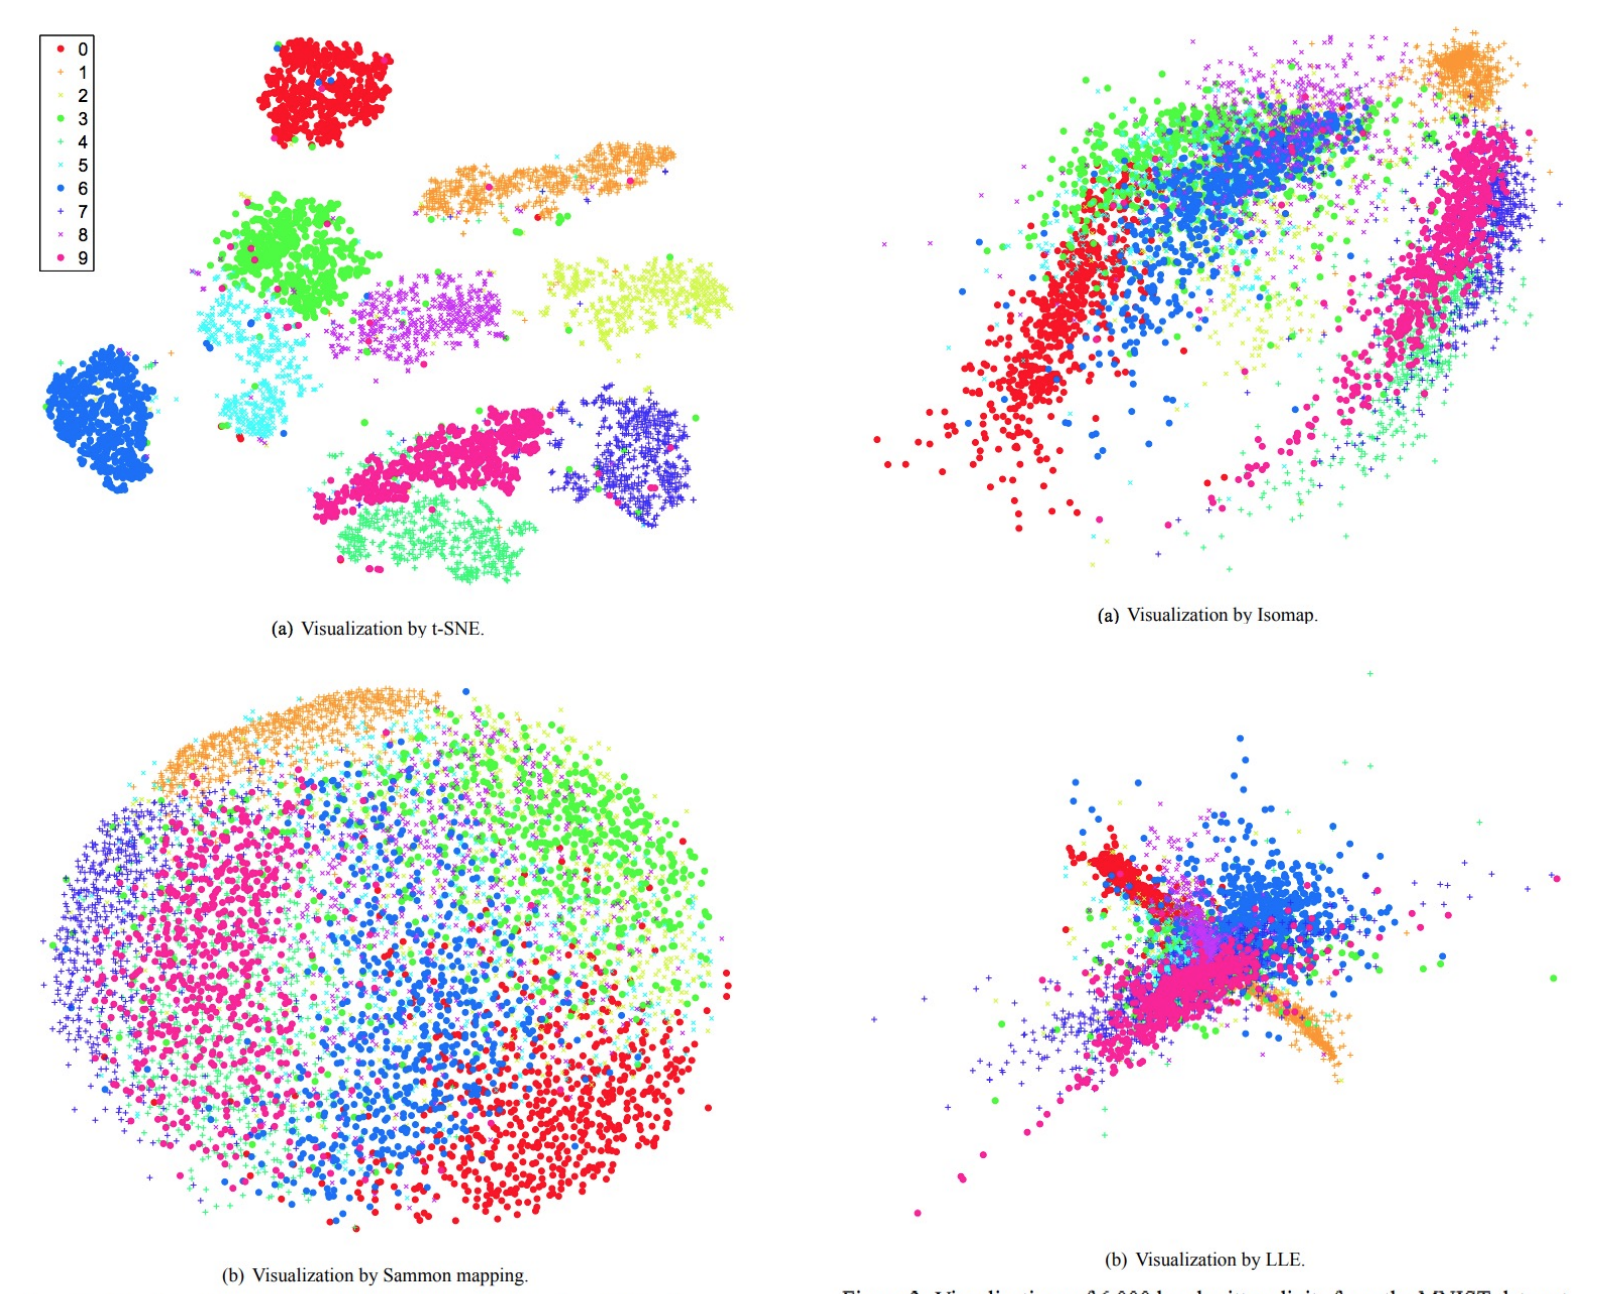
\includegraphics[scale=0.28]{chapter_7/files/fig3.png}
    \captionof{figure}{Comparing visualization results on MNIST
      dataset between tSNE, Sammon mapping, Isomap, and LLE.} 
\end{center}

Yet tSNE does have a few caveats and limitations. First, the
perplexity parameter needs to be chosen carefully and might need
knowledge about some general knowledge about the data. Varying
perplexity can give drastically different visualizations that show
different structures, as the follwoing figure shows. 

\begin{center}
    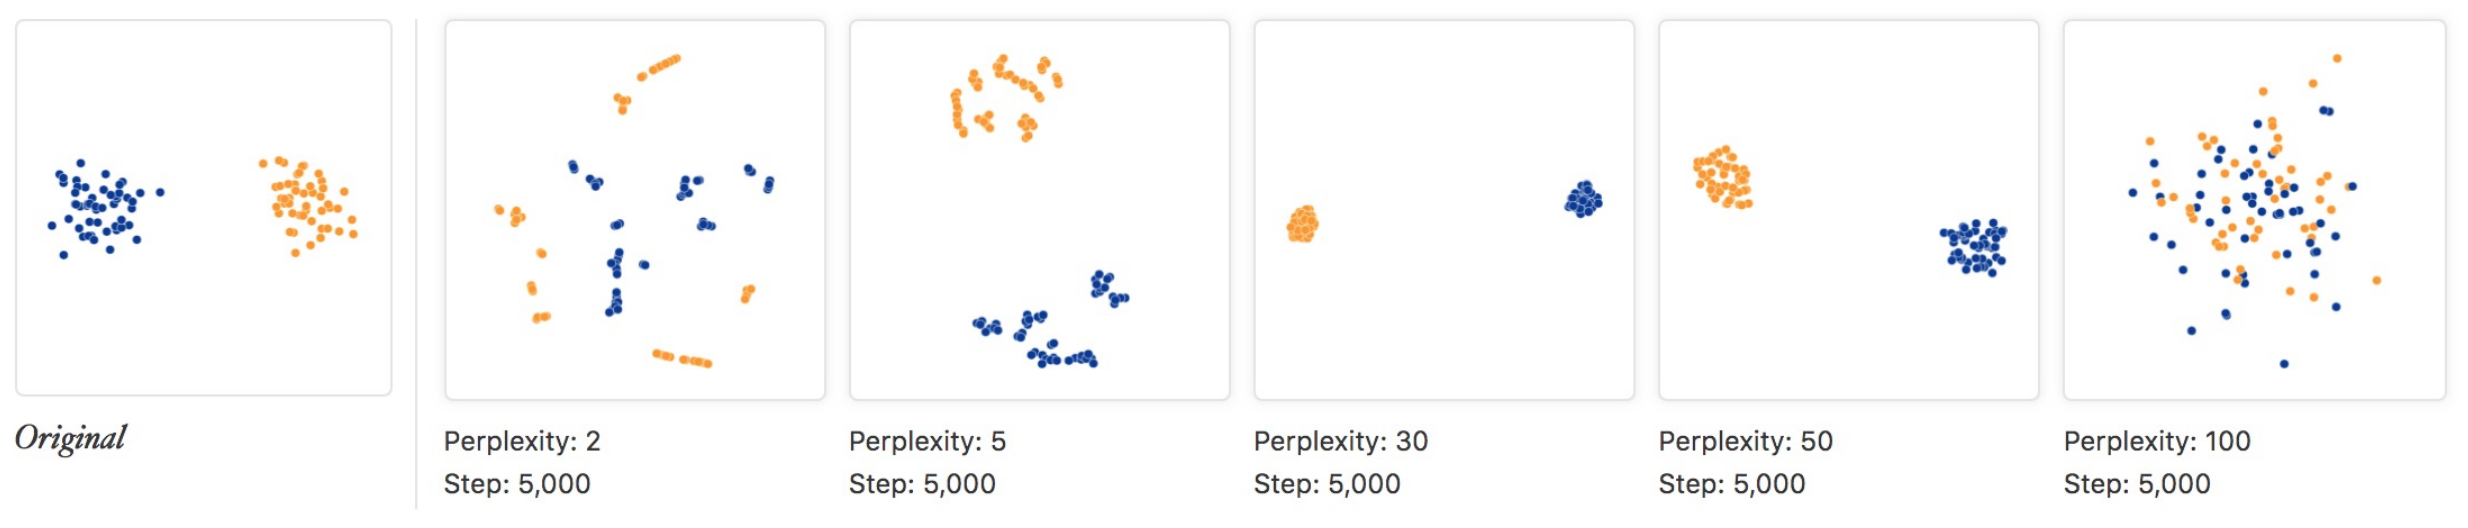
\includegraphics[scale=0.32]{chapter_7/files/fig4.png}
    \captionof{figure}{Impact of perplexity on resulting embeddings.}
\end{center}

Additionally, coordinates after embedding have no meaning. While tSNE
can preserve the general structure of data in the original space such
as clusters, it may distort those structure in the embedded 2D
space. Therefore, the embedded tSNE components carry no inherent
meaning and can merely be used for visualization. 

\begin{center}
    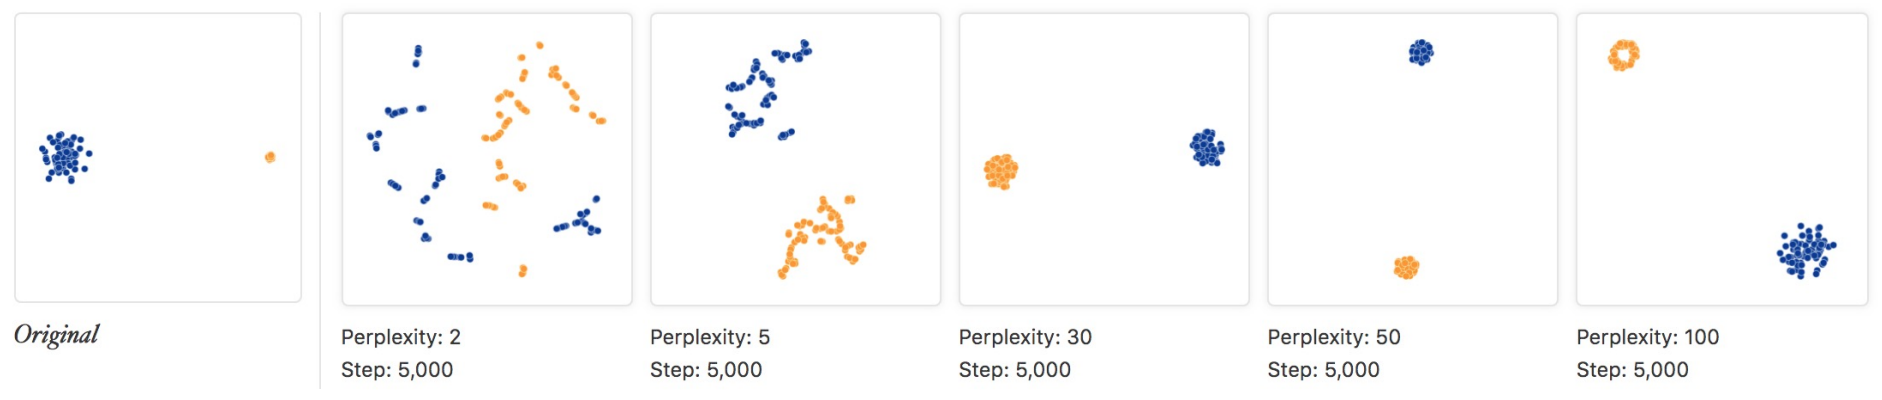
\includegraphics[scale=0.5]{chapter_7/files/fig5.png}
    \captionof{figure}{Size of clusters after embedding has no meaning
      like how they were in the original space.} 
\end{center}

Finally, since tSNE focuses on the local structure, the global
structure is only sometimes preserved. Consequently, interpretation of
the relationship between clusters cannot be obtained from tSNE
embedding alone. 

\begin{center}
    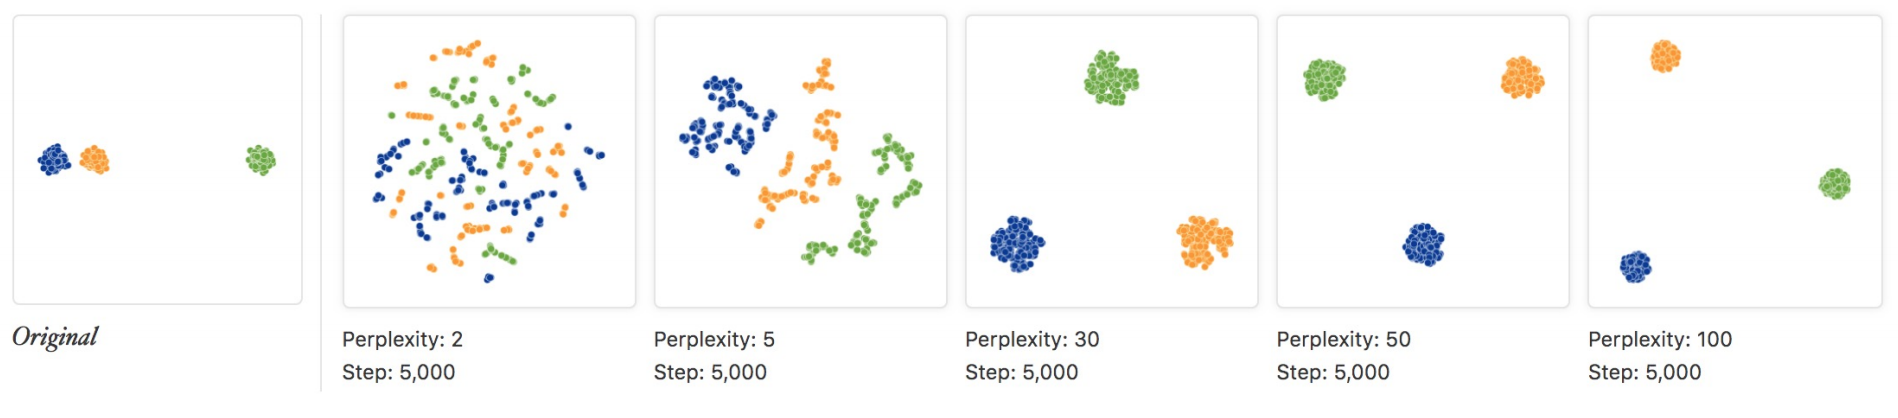
\includegraphics[scale=0.5]{chapter_7/files/fig6.png}
    \captionof{figure}{tSNE fails to capture the fact that blue and
      orange clusters are closer to each other than to the green
      cluster.} 
\end{center}

With these three caveats in mind, we conclude the limitations of tSNE.
\begin{itemize}
  \item tSNE can sometimes create extra (spurious) clusters. However,
    if the density of clusters in the higher dimension is constant, then
    tSNE will work and give the same number of clusters.
  \item tSNE does not work well for general dimensionality problem
    where the embedded dimension is greater than 2D or 3D but the
    meaning of distances between points needs to be preserved as well
    as the global structure. 
  \item Curse of dimensionality (tSNE employs Euclidean distances
    between near neighbors so it implicitly depends on the local
    linearity on the manifold) 
  \item $O(N^2)$ computational complexity
  \item Perplexity number, number of iterations, the magnitude of
    early exaggeration parameter have to be manually chosen 
\end{itemize}

\newpage
\subsection{Theoretical Guarantee}
Before we present recent theoretical results on tSNE, we need to first
formally define visualization. 
\begin{definition}[Visible Cluster]
    Let $\mathbf{Y}$ be a 2-dimensional embedding of a dataset
    $\mathbf{X}$ with ground-truth clustering $C_1,...,C_k$. Given
    $\epsilon \geq 0$, a cluster $C_l$ in $\mathbf{X}$ is said to be
    $(1-\epsilon)$-visible in $\mathbf{Y}$ if there exist $\mathbf{P},
    \mathbf{P_{err}} \subseteq [n]$ such that: 

    \indent (i) $\vert (\mathbf{P}\backslash C_l) \cup (C_l \backslash
    \mathbf{P}) \vert \leq \epsilon \cdot \vert C_l \vert$ i.e. the
    number of False Positive points and False Negative points are
    relatively small compared with the size of the ground-truth
    cluster.\\ 
    \indent (ii) for every $i,i' \in \mathbf{P}$ and $j \in [n]
    \backslash (\mathbf{P} \cup \mathbf{P_{err}})$, $\vert \vert y_i -
    y_{i'} \vert \vert \leq \frac{1}{2} \vert \vert y_i - y_j \vert
    \vert$ i.e. except some mistakenly embedded points, other clusters
    are far away from the current clusters.\\ 
    In such a case, we say that $\mathbf{P}(1-\epsilon)$-visualize
    $C_i$ in $\mathbf{Y}$. 
\end{definition}

\begin{definition}[Visualization]
    Let $\mathbf{Y}$ be a 2-dimensional embedding of a dataset
    $\mathbf{X}$ with ground-truth clustering $C_1,...,C_k$. Given
    $\epsilon \geq 0$, we say that $\mathbf{Y}$ is a
    $(1-\epsilon)$-visualization of $\mathbf{X}$ if there exists a
    partition $\mathbf{P}_1,...,\mathbf{P}_k,\mathbf{P}_{err}$ of
    $[n]$ such that:\\ 
    \indent (i) For each $i \in [k]$, $\mathbf{P}_i
    (1-\epsilon)$-visualizes $C_i$ in $\mathbf{Y}$.\\ 
    \indent (ii) $\vert \mathbf{P_{err}} \vert \leq \epsilon n$
    i.e. the proportion of mistakenly embedded points must be
    small.\\ 
    When $\epsilon = 0$, we call $\mathbf{Y}$ a full visualization of
    $\mathbf{X}$. 
\end{definition}

\begin{definition}[Well-separated, spherical data]
Let $\mathbf{X}=\{ x_1,...,x_n \} \subset \mathbb{R}^d$ be clusterable
data with $C_1,...,C_k$ defining the individual clusters such that for
each $l \in [k]$, $\vert C_l \vert \geq 0.1(n/k)$. We say that
$\mathbf{X}$ is $\gamma$-spherical and $\gamma$-well-separated if for
some $b_1,...,b_k > 0$, we have:\\ 
\indent (i) $\gamma$\textbf{-Spherical}: For any $l \in [k]$ and $i,j
\in C_l (i\neq j)$, we have $\vert \vert x_i -x_j \vert \vert^2 \geq
\frac{b_l}{1+\gamma}$, and for $i \in C_l$ we have $\vert \{ j \in C_l
\backslash \{ i\} : \vert \vert x_i - x_j \vert \vert^2 \leq b_l \}
\vert \geq 0.51 \vert C_l \vert $i.e. for any point, points from the
same cluster are not too close with it and at least half of them are
not too far away.\\ 
\indent (ii) $\gamma$\textbf{-Well-separated}: For any $l, l' \in
        [k](l\neq l'),i\in C_l$ and $k\in C_l'$, we have $\vert \vert
        x_i - x_j \vert \vert^2 \geq (1+\gamma \log n)\max \{ b_l,
        b_{l'}\}$i.e. for any point, points from other clusters are
        far away.\\ 
\end{definition}

\noindent Given the above definitons, Arora et al. have proven the
following results 
\begin{theorem}
    Let $\mathbf{X}=\{ x_1,...,x_n\} \subset \mathbb{R}^d$ be a
    $\gamma$-spherical and $\gamma$-well-separated clusterable data
    with $C_1,...,C_k$ defining k individual clusters of size at least
    $0.1(n/k)$, where $k<< n^{1/5}$. Choose $\tau^2_i =
    \frac{\gamma}{4} \cdot \min_{j\in [n]\backslash \{ i\}} \vert
    \vert x_i - x_j \vert \vert^2 (\forall i \in [n])$, step size
    $h=1$, and any early exaggeration coefficient $\alpha$ satisfying
    $k^2 \sqrt{n}\log n << \alpha << n$.\\ 
Let $\mathbf{Y}^{(T)}$ be the output of t-SNE after $T=\Theta
(\frac{n\log n}{\alpha})$ iterations on input $\mathbf{X}$ with the
above parameters. Then, with probability at least 0.99 over the choice
of the initialization, $\mathbf{Y}^{(T)}$ is a full visualization of
$\mathbf{X}$. 
\end{theorem}

\begin{corollary}
Let $\mathbf{X}=\{ x_1,...,x_n \} $ be generated i.i.d. from a mixture
of k Gaussians $\mathbf{N}(\mu_i, \mathbf{I})$ whose means
$\mu_1,...,\mu_k$ satisfy $\vert \vert \mu_l - \mu_{l'} \vert \vert =
\tilde{\Omega} (d^{1/4})$($d$ is the dimension of the embedded space)
for any $l\neq l'$.\\ 
Let $\mathbf{Y}$ be the output of the t-SNE algorithm with early
exaggeration when run on input $\mathbf{X}$ with parameters from
Theorem 3.1. Then with high probability over the draw of $\mathbf{X}$
and the choice of the random initialization, $\mathbf{Y}$ is a full
visualization of $\mathbf{X}$. 
\end{corollary}

The proof of the above results is rather extensive, and the following
road map outlines steps of the whole proof. For detailed proof, see
the original paper by Arora et al. 

\begin{center}
    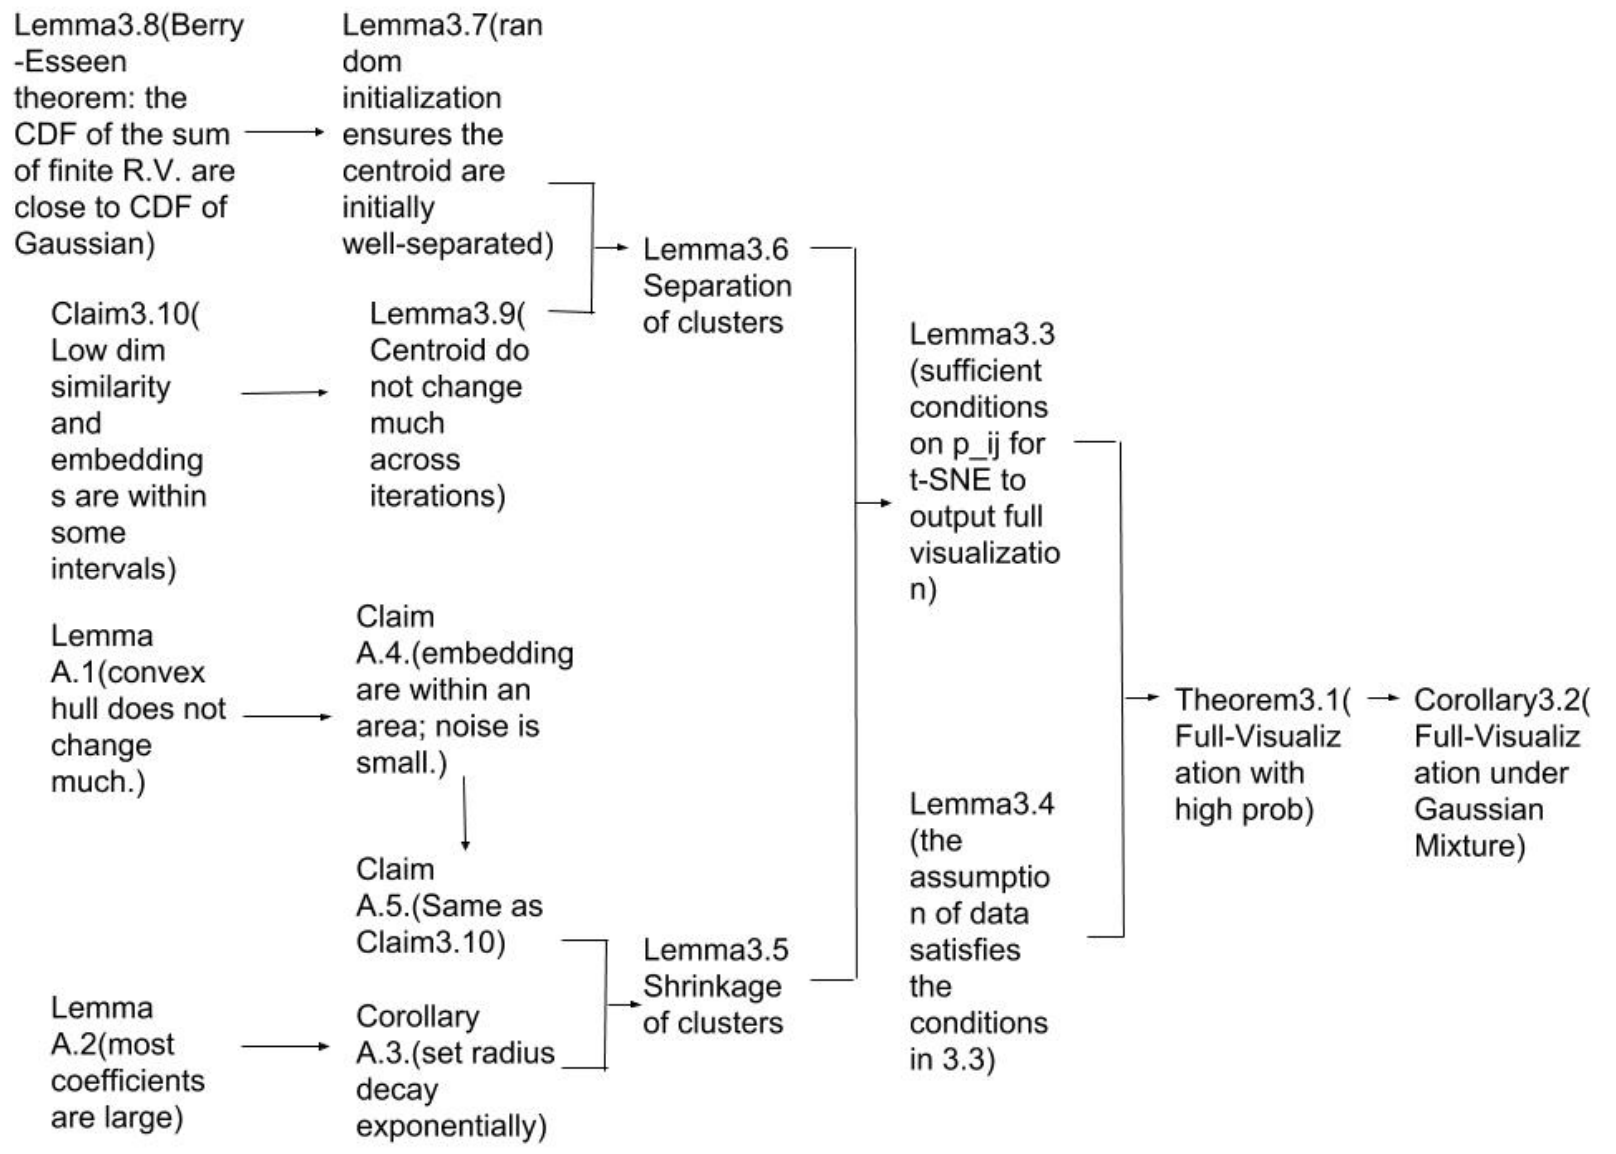
\includegraphics[scale=0.5]{chapter_7/files/fig7.png}
    \captionof{figure}{Proof road map. The numbering of lemmas,
      corollaries, and theorems correspond to that used in the
      original paper.} 
\end{center}
